% ----------------------------------------------------------------------

\begin{savequote}[50mm]
If you live among wolves you have to act like a wolf.
\qauthor{Nikita Khrushchev}
\end{savequote}


\chapter{Remote Actuation}
\label{cha:actuate}


\newcommand{\restdesc}{\emph{RESTdesc}}
\newcommand{\spaceActuation}{\emph{Space-based actuation}}
\newcommand{\restActuation}{\emph{REST actuation}}
\newcommand{\hybridActuation}{\emph{Hybrid actuation}}


% the code below specifies where the figures are stored
\ifpdf
    \graphicspath{{\pathchapsix/figures/PNG/}{\pathchapsix/figures/PDF/}{\pathchapsix/figures/JPG/}{\pathchapsix/figures/}}
\else
    \graphicspath{{\pathchapsix/figures/EPS/}{\pathchapsix/figures/}}
\fi


%------------------------------------------------------------------------- 


In the previous chapter, we presented an energy-aware technique to search on the completely distributed semantic space. % technique, mechanism???
%This search mechanism promotes the end-to-end interaction between the objects.
However, acting over an \ac{ubicomp} environment is as important as observing what happens on it.
Although this dissertation describes this problem less thoroughly, we consider interesting to discuss it to provide the complete story. %not leave loose ends. % transmit a broader vision. % the big picture

\bigskip

This chapter presents and compares two techniques to change the physical environment.
The first technique is based on common \ac{ts} usage patterns while the second one relies on semantically described \ac{rest} services to create a plan to fulfil a given goal.
The rest of this chapter refers to them as \spaceActuation{} and \restActuation{} respectively.

Note that the second actuation technique is out the scope of the space-based communication covered in this dissertation.
However, the seamless integration of these \ac{rest} services opens the door to reuse the capabilities of many existing devices.
Therefore, we propose reusing the \acs{http} \acsp{api} of already existing semantically described providers.
% without adapting them to the space-based computation. % a nivel practico hacemos más fácil empezar a usar nuestro middleware

This chapter explores this reuse helped by a simple real-world scenario.
The goal of the scenario is to remotely change the light of a lamp.

\bigskip

This chapter is organized as follows.
Sections \ref{sec:actuation_space} and \ref{sec:direct_actuation} present the two techniques and their corresponding implementations of the baseline scenario\footnote{
The implementations of the baseline scenario have been made public at \url{XXX}. % TODO TODO TODO Update the URL.
\label{fn:impl_available}
}.
Section~\ref{sec:hybrid_actuation} compares these techniques and explores how they can interoperate. % no funciona en ambos sentidos, igual habría que especificarlo!
This exploration is done by means of a new implementation\footref{fn:impl_available} which reuses much of the implementations from sections \ref{sec:actuation_space} and \ref{sec:direct_actuation}.
%Specifically, it presents a consumer willing to indirectly actuate through a space in a semantically described \acs{http} provider. % no sé si queda muy claro
After that, Section~\ref{sec:actuation_discussion} discusses the advantages and limitations of the previous implementation presenting further implementation alternatives.
Finally, Section~\ref{sec:actuation_summary} concludes the chapter.


% ----------------------------------------------------------------------


\section{Space-based actuation}
\label{sec:actuation_space}

% explicar brevemente patrones
% requirements: sistema de suscripciones (out of the scope)
% escenario de ejemplo en Ubicomp

This section presents the first technique to change the physical environment.
That technique is space-based, i.e., participants coordinate by reading and writing into a shared \Space{}. % that y no this, para no confundir con la que se presenta en esta sección
This encourages an uncoupled communication between applications using the same \Space{}.

Section~\ref{sec:ts_patterns} briefly describes \acl{ts}'s most common application patterns and discusses which ones are suitable for \ac{ubicomp} environments. % according to the classification of \citet{freeman_javaspaces_1999}.
These patterns constitute the base of what we called \spaceActuation{}.
Section~\ref{sec:notification} presents the \spaceActuation{}'s core requirement: a subscription mechanism.
Finally, Section~\ref{sec:actuation_scn1} explains how to implement the baseline scenario according to the space usage patterns. % más que usage pattern, igual es app pattern


\subsection{Background}
\label{sec:ts_patterns}

According to \citet{freeman_javaspaces_1999}, there are four main application patterns which can be used in \ac{ts}:

\begin{description}
  \item[Replicated-worker pattern.] In this pattern, there is a master process and many worker processes able to compute the same task.
				    %% REDUCIENDO esto: %%
%				    The master takes a problem and divides it in tasks which are solved by any of the workers.
%				    More concretely the pattern is composed by the following steps:
% 				    \begin{enumerate}
% 				      \item The master divides a problem up into smaller tasks.
% 				      \item It writes them in the space.
% 				      \item Any of the many workers takes a task.
% 				      \item That worker computes the task.
% 				      \item It writes the result of that computation.
% 				      \item The master collects the results for the tasks it wrote.
% 				      \item Once the master has all the results, it combines them into a meaningful overall solution.
% 				    \end{enumerate}  
				    The master takes a problem, divides it into smaller tasks, and writes these tasks into the space.
				    Any available worker takes a task, processes it, and writes the result back into the space.
				    When all the workers have written their results, the master takes these results and combines them into a meaningful merged solution.
				    %Note that the workers accept new tasks whenever they are available and able to work.
				    %Therefore, while a worker is busy computing a big task, another one can solve many small tasks.
				    %In other words, this pattern naturally \emph{balances the load} on the space.
				    %Besides, it is \emph{scalable} since we can add more workers running in more machines without rewriting our code.
				    This pattern is scalable and naturally balances the load on the space.
  \item[Command pattern.] This pattern encapsulates the behaviour into the tuples shared in the space.
			  Therefore, it requires 
			  \begin{enumerate*}[label=\itshape(\arabic*\upshape)]
			    \item to share behaviour through the space, and
			    \item any generic worker to be able to compute the behaviour.
			  \end{enumerate*}
			  % nosotros pasamos de este jaleo
			  %For instance, a graph in \ac{tsc} could include code in an interpreted programming language. % elucubrar sobre esto sólo liaría
			  %In that way, a generic worker application can compute whatever code other processes define and share through the space.
			  %This pattern is only possible in \aclp{ts} where the behaviour can be described generically (e.g., in object-oriented \acp{ts}).
			  %Furthermore, the tasks to be performed over \ac{ubicomp} environments are not generically processable by any node.
			  %In contrast, each device is responsible of managing its own actuators on behalf of the rest.
			  %Therefore, this pattern will not be considered.
  \item[Marketplace pattern.] In this pattern, producers (or sellers) and consumers (or buyers) of resources interact to find the best deal. % TODO cita TripCom?
			  %It should be noted that the resources are products or services which can be bought and sold.
			  %Therefore, it is not applicable to the environments considered. % o use cases
			  %esto está relacionado con el paper aquel de TripCom y con el de Simon de hace un año en WoT
  \item[Specialist patterns.] In contrast to the replicated-worker pattern, in this pattern, each worker is specialized.
                              Therefore, each worker performs a particular task.
                              \citeauthor{freeman_javaspaces_1999} enumerate three subtypes:
			      \begin{description}
				  \item[Blackboard pattern.]
					It associates the concept of the space to a \emph{blackboard}.
					Following this analogy, the master is associated with a teacher, tasks with \emph{problems} and the specialized workers with \emph{students}.
					The blackboard pattern starts when the \emph{teacher} writes a \emph{problem} in the \emph{blackboard}.
					The \emph{students} observe the space and write their intention to contribute to solve the problem (i.e., \emph{raise their hands}).
					The \emph{teacher} selects an expert which will make a modification.
					After the modification, the \emph{teacher} decides if it has found the solution or another \emph{student} should contribute.
				  \item [Trellis pattern.]
					In this pattern, the master arranges the problem into low-level, mid-level, and high-level pieces.
					The workers of each level benefit from the refined data provided by the immediate level below.
				  \item [Collaborative patterns.]
					It encompasses all the patterns which allow nodes to collaborate to complete a greater task (i.e., by creating a workflow).
					%They are specific to the domain so they cannot be generalized, but it includes all the patterns where the nodes collaborate to complete a greater task
					%(e.g., by creating a workflow).
			      \end{description}
\end{description}


% Voy preparando el terreno para que se vea que los primeros son más de computación y el otro de negociación
To summarize, the \emph{replicated-worker pattern} is centred in optimizing the computation by parallelising tasks.
The \emph{command pattern} can be seen as an abstraction of the latter where the behaviour is shipped in the tuples.
The \emph{marketplace pattern} allows negotiation of two entities through the space.
% Coño! pero si el especialista te permite colaborar...
Finally, the \emph{specialist pattern} allows nodes with distinct capabilities to cooperate towards a common goal.


% Posibilidad: Un esquema dividido en 4 en el que aparecen todos los patrones explicados.
%   No es fácil mostrar el 2do y el 3ero.
%   Una intentona de estos y otros patrones inventados en Lancaster:
%      https://docs.google.com/a/deusto.es/document/d/1QXGsQ4-wAByc_ByQ-Tts-TSphSQAzfO_c3mcgoZdloc/edit


% \subsection{Envisaged Scenarios}
% \label{sec:envisaged_scenarios}

% This section devises two stereotypical scenarios for home automation.
% Section~\ref{sec:envisaged_scn1} presents a scenario which regulates the temperature of a smart environment (e.g., a home or office) according to the user preferences.
% Section~\ref{sec:envisaged_scn2} describes a smart environment which warns the user using different mechanisms to help him avoid a sedentary lifestyle.


% Both scenarios emphasize how devices can coordinate in a decoupled mode using the patterns seen in the previous section. % más de uno?
Regarding the application of these patterns to \ac{ubicomp}, we observed that:
% si hace falta argumento de autoridad, se puede comentar que esto emana de nuestra experiencia en distintos proyectos.
\begin{itemize}
  \item Devices in \ac{ubicomp} often serve to very specific and local needs.
        For example, let us imagine a mobile phone showing a message or an embedded device turning on the air conditioning of a room.
        %Although there may exist some redundancy in the tasks which different nodes can be accomplish, the task are not nodes are not as interchangeable as in... son tareas simples, no necesitan optimizar ni lanzar muchas
  \item These tasks are usually lightweight. % do not require a lot of computation resources.
	% Contrasta con TripCom, que manejaba servicios web potencialmente pesados y que crearon un sistema (WSMX)
        They intent to achieve concrete and simple goals which usually imply more I/O operations than processing ones.
\end{itemize}
Therefore, \ac{ubicomp} generally faces a problem of collaboration between nodes with different capabilities.
In this problem, computation or negotiation aspects are secondary. % se entenderá a qué me refiero con computation??
Consequently, we believe that the \emph{specialist patterns} fit \ac{ubicomp} needs best.

% \subsubsection{Scenario 1: Temperature Regulation}
% \label{sec:envisaged_scn1}
% 
% The first scenario presents a room populated with several kind of sensors such as Oracle's SunSPOTs \citeweb{sunspot},
% % Si se recupera esto, habría un TODO de referenciar a la parte donde se hayan referenciado bien los dispositivos! (e.g., see ~\ref{environment})
% % Para el resto proveer al menos una URL!
% Digi's XBee sensors with an IP gateway,
% the sensors on a KNX domotic bus \citeweb{knx}, and a fan connected to a FoxG20 \citeweb{foxg20} embedded platform as an actuator (see Figure \ref{fig:devices_scenario}).
% In addition, an Android application \citeweb{android} semantically stores the temperature preferences of the user.
% 
% 
% \InsertFig{devices_scenario}{fig:devices_scenario}{
%   The devices used in the devised scenarios.
% }{
% }{0.7}{}
% 
% 
% An independent node (i.e., the master node) continuously reads from the space % using \emph{read primitive}
% \begin{enumerate*}[label=\itshape(\arabic*\upshape)]
%   \item the room's temperature, and
%   \item the user's desired temperature.
% \end{enumerate*}
% Note that the master node does not care about who exactly provides the temperature information.
% It just takes the first available graph from the space.
% When the second one is below the first one, it generates a ``\emph{decrease temperature during a certain period}'' task which can be consumed by different independent worker nodes.
% In this case, the FoxG20 periodically checks for orders it can fulfil extracting them from the space. % consumes them with a \textit{take primitive}.
% % zasca, acabamos de poner en bandeja que nos rechine lo de comprobar periodicamente
% 
% 
% 
% \subsubsection{Scenario 2: Sedentary Lifestyle Checker}
% \label{sec:envisaged_scn2}
% 
% The second scenario presents an application which helps the user to avoid a sedentary lifestyle by giving him different warnings.
% We consider the recommendation that states that an adult should walk at least 10.000 steps in an ordinary day \citep{tudor2002taking}.
% Taking into account the expected steps which should have been completed at each moment of the day, the application generates different priority level messages.
% 
% There are several nodes involved in this task.
% Each node runs on a device. % which belongs to a user.
% First, an Android phone periodically updates the number of steps covered by a user that day \citeweb{pedometer}.
% %Besides, it writes her profile, more important to this problem: her age. % simplificado un poquillo
% Second, there is an undefined number of devices which know how to warn the user about her unhealthy behaviour.
% Third, there is a node in charge of generating the warnings.
% 
% 
% \medskip
% 
% 
% The application follows the \emph{blackboard pattern}.
% The node which generates the warnings resembles a \emph{teacher}.
% Each warning for a user resembles a \emph{problem} for the students.
% Finally, the \emph{students} are allegorically represented by the devices which can warn the user.
% % IG: no es nada intuitivo. Leyendo despues lo entiendo, pero... es raro
% % AG: reescrito para hacer ver que hablo de una metafora/analogía/alegoría
% 
% 
% When the \emph{teacher} writes a warning for a user, the devices able to warn the user write information about themselves into the space.
% This information helps the teacher to select the most appropriate \emph{student} for each task.
% In this example, the devices write their ownership and the intrusiveness level of their warning method.
% The \emph{teacher} reads these characteristics, chooses a \emph{student} to solve the \emph{problem} and updates the \emph{problem} to indicate the selection.
% %If no device writes their characteristics, the \emph{teacher} can wait longer.
% Then, the selected device takes any warning for it and warns the user. % no tiene respuesta
% If the chosen device does not take the message in a time span, the \emph{teacher} can update the \emph{problem} with a new selection.
% 
% 
% With this application, if the priority level is low, the user receives the warning in a less intrusive way.
% For example, room's light brightness can be increased for low priority notifications, a Chumby \citeweb{chumby} can show an icon for normal priority ones and the user's mobile phone show directly the message when it is a high priority warning. % IG: yo anyadiria una tablita para los dos scenarios mostrando los actuadores y los niveles. Aqui esto me salta un poco de repente.
% The remarkable characteristic of this mechanism is that the devices present in the environment at each moment can vary and the application will still fulfil its goal.


\subsection{Notification mechanism}
\label{sec:notification}


In the patterns described in the previous section, some writings in the space trigger other node's action.
For example, a device might show a message whenever a new warning is written into the space. % e.g., a task or a result
To be aware of these writings, the node can either poll the space or rely on a notification mechanism. % async or blocking
Obviously, the later leads to a more efficient use of the network. % is closer to optimal and more scalable approach.


As a consequence, a notification mechanism is highly advisable to fulfil \ac{ts}'s application patterns in a distributed environment.
Although the implementation of this notification mechanism is beyond the scope of this thesis,
% Hablar de requisitos, describir nuevas primitivas de suscripciones o alternativas de implementación
it should comply with the following aspects:
\begin{itemize}
  %  Debe permitir polling (sync), por ello proponemos nuevas primitivas: read_async y take_async.
  \item Do not substitute the pull-based search. % porque todavía puede ser interesante en otros casos
        The middleware must provide additional \emph{read} and \emph{take} primitives.
  % Se evalúan sobre el espacio, no sobre el outer-space. 
  \item Since the notification mechanism intends to allow coordination patterns,
        it must consider the knowledge from the \coordspace{}. % TODO comprobar que lo llamé así en el anterior capítulo
        In other words, knowledge from the \outerspace{} will not trigger notifications. % TODO usar constante para esto
  % Evaluarse cada X, no siempre que se escriba algo o se vuelve loco.
  \item The evaluation of the subscriptions must not interfere with the writing process (e.g., introducing a delay).
        Therefore, it must run asynchronously.
  % Debe ser sencillo de implementar por cualquier nodo. Para ello proponemos un mínimo contrato: callback URL.
  \item Ease its adoption by any type of computing platform.
	This can be achieved by reducing the requirements on the \emph{clients}.
        For instance, a callback \ac{url} passed during the subscription can represent a minimal contract between the client and the server. % no viceversa
  % Deben caducar para no mantener suscripciones de dispositivos que ya no existen.
  \item Provide additional subscription removal mechanisms.
	\ac{ubicomp} scenarios are composed by unreliable devices which may frequently join and leave the space.
	In this situation, the correct use of unsubscription primitives cannot be guaranteed.
	This may worsen the performance of the system with useless subscriptions from absent devices.
	Therefore, the device managing the subscriptions should adopt more proactive mechanisms.
	For example, it may let the subscriptions expire after a lifetime or remove them when it discovers the unavailability of a callback \ac{url}. % algo así como garbage collection
	% A) The subscriptions must expire.
        % The expiration will allow to delete subscriptions from absent devices. % no longer present devices
        % This also implies that clients are responsible for periodically updating their subscriptions.
        % B) Additional mechanism
        % For instance, a \emph{garbage collection} agent can check the availability of callback \acp{url}.
        % For unavailable callback \acp{url}, the subscriptions can be removed.
\end{itemize}


The main drawback of any subscription mechanism is that it breaks the \acl{rests} property of the \ac{rest} style.
According to Section~\ref{sec:network_properties}, this implies that network performance will improve at the cost of scalability, simplicity and reliability.


\subsection{Baseline scenario: Implementation 1}
\label{sec:actuation_scn1}
\newcommand{\implSpace}{\emph{Implementation 1}}

This section describes how to implement the baseline scenario using the \spaceActuation.
The implementation presents the following nodes:
\begin{enumerate}[label=\itshape(\Alph*\upshape)] % o \itshape(\Alph*\upshape~node)
  \item A node which reacts to the tasks written into a shared semantic space.
	The node running this implementation is aware of the tasks written into the space and changes the light's value accordingly. % esto es, se suscribe a ellas
	Figure~\ref{fig:flow_space_prov} shows the initialisation of this node and the process performed when a graph is detected.
	
  \item A node which writes tasks into a shared semantic space describing its desire to change the light's value.
	Figure~\ref{fig:flow_space_cons} shows the actions taken by this node.
	As it can be seen, the process is divided in two temporarily independent processes.
	The first writes the task and the second processes the result whenever it is written into the space.
	
  \newcounter{enumNodes}
  \setcounter{enumNodes}{\arabic{enumi}}
\end{enumerate}

% In advance, we will refer to these nodes as "A" and "B" using the following commands:
\newcommand{\nodeProvSpace}{\emph{Node A}}
\newcommand{\nodeConsSpace}{\emph{Node B}}


\begin{figure}
        \centering
	\subfigure[figtopcap][\nodeProvSpace] {
                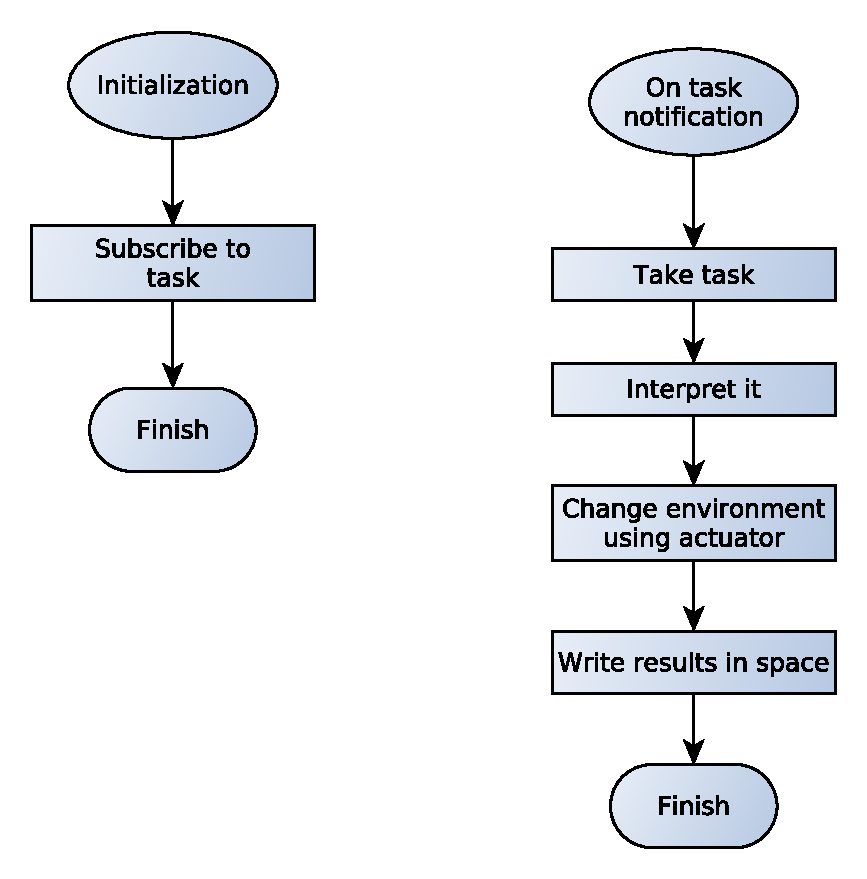
\includegraphics[width=0.45\linewidth]{flowSpaceProvider}
                \label{fig:flow_space_prov}
        }
	~ %add desired spacing between images, e. g. ~, \quad, \qquad etc.
          %(or a blank line to force the subfigure onto a new line)
	\subfigure[figtopcap][\nodeConsSpace] {
                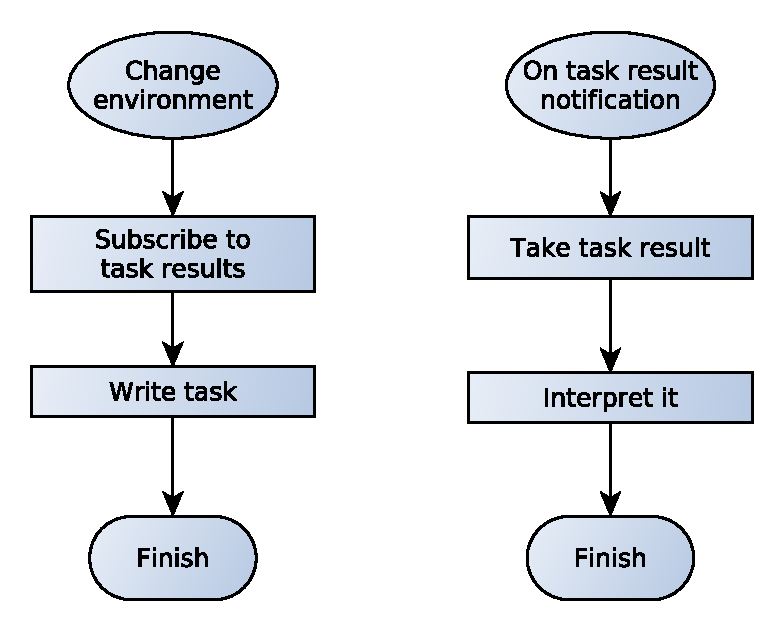
\includegraphics[width=0.45\linewidth]{flowSpaceConsumer}
                \label{fig:flow_space_cons}
        }
        \caption{Flow charts for \nodeProvSpace{} and \nodeConsSpace{}}
        \label{fig:flow_space}
\end{figure}


\nodeProvSpace{} first subscribes to changes in the space (see Listing~\ref{lst:task_subscription}).
Then, \nodeConsSpace{} writes a task to be performed (see Listing~\ref{lst:task}) and subscribes to its result.
As a consequence of the writing, \nodeProvSpace{} reacts by taking the task, interpreting it, changing the environment through its actuator and writing the result.
Finally, \nodeConsSpace{} gets a notification of the written result, takes it and processes it.


\begin{listing}
  \expandafter\def\csname PY@tok@err\endcsname{}
{\small
\begin{Verbatim}[commandchars=\\\{\},numbers=left,firstnumber=1,stepnumber=1]
\PY{k}{select }\PY{n+nv}{?value }\PY{k}{where}\PY{p}{\PYZob{}}
\PY{n+nv}{  ?observation}\PY{o}{ a }\PY{n+na}{frap:Preference }\PY{p}{;}
	\PY{o}{a }\PY{n+na}{ssn:ObservationValue }\PY{p}{;}
	\PY{o}{dul:isClassifiedBy  }\PY{n+na}{ucum:lux }\PY{p}{;}
	\PY{o}{dul:hasDataValue }\PY{n+nv}{?value }\PY{p}{.}
\PY{p}{\PYZcb{}}
\end{Verbatim}
}

  \caption[Subscription to light preferences]{Subscription to light preferences written into the space.}
  \label{lst:task_subscription}
\end{listing}


% dar detalles de cómo se ha implementado
To simplify the implementation of the scenario, we consider a purely centralized space with a subscription mechanism.
% subscripciones SPARQL
This mechanism uses \acs{sparql} \citeweb{sparql2008} and defines two different primitives.
The first one takes into account the knowledge from the last graph written to trigger the notifications.
% http://english.stackexchange.com/questions/2981/alternatives-to-computationally-expensive
The second primitive considers the knowledge from the whole space and hence is more computationally costly.


\begin{listing}
  \expandafter\def\csname PY@tok@err\endcsname{}
\begin{Verbatim}[commandchars=\\\{\},numbers=left,firstnumber=1,stepnumber=1]
\PY{n+nc}{:obsv} \PY{o}{a} \PY{n+na}{ssn:ObservationValue}\PY{p}{,} \PY{n+na}{frap:Preference} \PY{p}{;}
      \PY{n+nf}{dul:isClassifiedBy}  \PY{n+na}{ucum:lux} \PY{p}{;}
      \PY{n+nf}{dul:hasDataValue} \PY{l+m+mi}{21} \PY{p}{.}
\end{Verbatim}

  \caption[Task to set the light level in a space]{Task to \emph{set} the light level in a space. Note that the preference is conceptually equivalent to a task.}
  \label{lst:task}
\end{listing}


% TODO Posiblemente haya que cargarse esto porque no encaja...

\subsubsection{Actuation modelling}

% explain why like this? why not directly sensors/light?
The most abstract way to actuate on the environment would be to invoke a change referring to the sensed values.
For example, stating ``set \emph{Room A}'s light-level to 19 luxes''.
This would require the coordination of all the actuators which directly or indirectly affect this value.
Following the example, the lamps in \emph{Room A} and the curtains of \emph{Room A}'s windows should coordinate to give the exact desired value.


Even in this case, many other physical aspects would affect the value.
For instance, the daylight at each time of the day or the location of the light sensor.
As a consequence, we opt for clearly distinguishing between actuators and sensors.
In our implementations, the data measured by the sensors can only be indirectly affected by the actuators.


These indirect effects on the sensed values can be modelled for each actuator.
For example, to state that switching on a lamp increases the light measured by a sensor.
However, precisely anticipating the exact value of the new measure is difficult if not impossible due to the mentioned external physical conditions.
Considering this difficulty to predict their relationship and its tangential importance for the baseline scenario's implementations, we simply ignore these relationships.
We assume that the consumer previously determined which actuators it should change to fulfil its initial abstract goal.


\subsubsection{Ontologies used}

% Ontologies used
% explicar por qué hemos modelado así los escenarios?
The \emph{glue} between the two actuation worlds presented in this chapter is their data.
Therefore, the implementations presented in this chapter represent the environment according to the same ontologies. % u ontologías distintas con mapeo, pero paso de explicar eso.
This section provides the rationale behind the selection of the ontologies used.
% This selection does not pretend to be the best choice.


% por qué con medidas?
To represent the value of a lamp actuator, we use the SSN ontology \citeweb{ssn}.
For example, we express that ``the lamp actuator has a light value of \emph{N} luxes''.
The SSN ontology is intended to describe measures for sensors, so its use for actuators can sound contradictory.
Note how the previous statement differs from ``the light sensed by a sensor located near the lamp has a value of \emph{N} luxes''.
However, to the best of our knowledge, there is no more widely-accepted ontology to specifically describe actuators.


% por qué uso preferencias?
The preferences ontology is another core ontology used in our implementations.
It is used to clearly distinguish between the value of an actuator and a consumer's intention or desire to change it.
A preference can turn into an actuator's new state, but it is not always necessarily true.
The actuator can discard a preference due to an usage policy, a malfunction or any other reason.

% por qué no se tienen en cuenta otras características como la localización o lo que sea => por simplificar
%   en el goal se podrían describir
\section{REST actuation}
\label{sec:direct_actuation}


The actuation technique presented in the previous section uses the \Space{} (i.e. it is indirect).
This technique implies that the actuator must be aware of the \Space{}'s content.
For instance, a heater must check the space to find if a new desired temperature was written.
% lo podrá reusar a través de un intermediario
% interop era una de las cosas que queriamos cuidar
% y qué pasa con las soluciones REST que quieren usar lo nuestro?


% por qué? motivación: permitir a otras app integrarse en nuestro espacio
In contrast, this section presents a second technique which directly actuates in the environment without using any \Space{}.
A consumer following this technique directly uses \ac{rest} \acp{api}. % i.e. it is the client of these \ac{api} <-- se entiende esto o hace falta dar el salto entre consumer y client?
These \acp{api} expose the devices' capabilities to make physical changes in the environment.

However, this apparently simple mechanism hides a difficulty: the consumer needs to discern how to use these \acp{api} to make such changes.
According to the \ac{rest} principles, a client should navigate through the resources of an \ac{api} with no prior knowledge of it.
% Copiar esta explicación mejor de algún lado:
The client should 
\begin{enumerate*}[label=\itshape(\arabic*\upshape)]
  \item interpret the representations provided by the server and then
  \item choose the appropriate state transition from the hypertext according to its intention. % y su conocimiento básico del protocolo: CRUD
\end{enumerate*}
To do this, this section advocates for a semantic description of these \acp{api}' resources.

Section~\ref{sec:actuation_rest_background} briefly compares different alternatives to build semantic \ac{rest} \acp{api}.
Section~\ref{sec:restdesc} presents the selected alternative and Section~\ref{sec:actuation_scn2} implements the baseline scenario using it.



\subsection{Background}
\label{sec:actuation_rest_background}

As Section~\ref{sec:network_properties} explained, semantic representations do not include a native way to express the hypertext. % TODO realmente se explica?
To solve this, three solutions can be adopted:
% Unos proponen extender con ontologías
\begin{enumerate}
  \item To use an ontology to represent the hypertext \citep{kjernsmo_necessity_2012}.
  \item To embed the hypertext independently to the representations on the \ac{http} headers \citep{mark_web_2010}.
  \item To provide a description of the state changes each \ac{http} request triggers \citep{verborgh_functional_2012,verborgh_ijcs_2014}.
\end{enumerate}


The latter two enable to discover resources and state transitions without adding metadata to the representations.
This allows not only to describe semantic representations, but any type of formats.


\citeauthor{mark_web_2010}'s \citep{mark_web_2010} approach is extended by \citet{erik_profile_2013} to define how to embed additional semantics to process a resource representation.
\citet{erik_profile_2013} calls these additional semantics \emph{profiles} and identifies them using \acsp{uri}.


\citet{verborgh_ijcs_2014} present a more expressive solution which goes beyond simply describing a resource type.
It also allows to semantically describe the knowledge needed to use a concrete \acs{http} verb on a resource, and the content this request returns. % o precondition
The materialization of this proposal is called \restdesc{} \citep{verborgh_functional_2012}.
\citet{mayer_semantic_2013} use \restdesc{} in an environment populated by web-powered devices. % i.e. the \ac{wot}
This environment is analogous to the ones envisioned by this dissertation. % analogous/equivalent


\bigskip


We consider \restdesc{} the best current solution which helps to achieve truly \ac{rest}ful \acsp{api}.
Therefore, this chapter assumes that the \ac{http} \acsp{api} whose capabilities we want to reuse in our space model describe their \acsp{api} with \restdesc{}.


\subsection{\restdesc{}}
\label{sec:restdesc}

% TODO mirar si tiene cabida la mención de otros enfoques para describir recursos que no son muy RESTful
%Different ways exist to describe \ac{rest} services. % mencionar WADL, etc.?
% citar a donde se hable de \restdesc{} y así ya se empieza a explicar la solución de forma discreta.
\restdesc{} describes \acs{http} methods using rules expressed in the \ac{n3} language \citeweb{n32011}.
% he evitado explicar que las reglas tienen premisa y conclusión, porque me parece demasiado obvio
A rule's \emph{premise} expresses the requirements to invoke a \ac{rest} service.
A rule's \emph{conclusion} expresses both the \ac{rest} call that needs to be made and the description of that invocation result.


\citet{verborgh_functional_2012} suggest three complementary alternatives to discover descriptions.
The first and second alternatives use \ac{http} mechanisms: content negotiation and the \ac{http} OPTIONS verb.
Using content negotiation a client can obtain a dereferenceable link's representation which corresponds to the description. % puede ser comments#algo
Requesting a resource using the \ac{http} OPTIONS verb a client can obtain the description in the response body.
Finally, the third alternative is not \ac{http}-centric and it depends on repositories to store and retrieve the descriptions.
% En el paper los autores no justifican bien porque es last resort, así que paso de meterme yo en berenjenales
% This alternative should only be used as a last resort because it requires out-of-band information (e.g. the repository address and how to use it) to learn how to use an \acs{api}.
% it separates the description of the \acp{api} functionality from the \acp{api} themselves. % dificultando el descubrimiento de las APIs usando sólo ellas


\citet{verborgh_ijcs_2014} propose a service composition mechanism for Web \acp{api} using \restdesc{}.
This mechanism uses as inputs:
\begin{enumerate*}[label=\itshape(\arabic*\upshape)]
  \item an initial state,
  \item a goal state,
  \item Web \ac{api} descriptions using \restdesc{}, and
  \item optional background knowledge.
\end{enumerate*}
Each of these inputs are semantically expressed and therefore, they can be processed by standard \ac{n3} reasoners.
These reasoners generate proofs about how to achieve the goal starting from the initial state and using the rest of the inputs.
These proofs can be seen as steps that need to be made to reach a desired state.


Additionally, \citeauthor{verborgh_ijcs_2014} distinguish between pre-proof and post-proof.
The first, are those which assume that the execution of all \acs{api} calls will behave as expected.
The latter, can be seen as a \emph{revision} of the pre-proof.
It executes the Web \acs{api} of the pre-proofs and uses actual execution results to generate a new proof.


\subsection{Baseline scenario: Implementation 2}
\label{sec:actuation_scn2}
\newcommand{\implRest}{\emph{Implementation 2}}

% poner un diagrama que presente el escenario?
% En ppio no, porque sería muy sencillote, y el flujo del consumidor que es el complejo ya ha sido explicado.
The proposed implementation for the baseline scenario using \restdesc{} presents the following nodes:
\begin{enumerate}[resume,label=\itshape(\Alph*\upshape)]
  \setcounter{enumi}{\theenumNodes}
  \item A node which exposes the lamp and its actuators through a \ac{rest} \ac{api}.
	This \ac{api} is described using \restdesc{}. % REST API seguro 100%? por si acaso decir HTTP API?
	To physically change the light value, any client must send an \acs{http} request to the resource which represents the light actuator.
	% Please note that \nodeProvRest{} is omitted because its operation is the usual for an \acs{http} server.
	
  \item A node which directly communicates with the desired provider.
	To discern which provider's resources has to call and how to do it, this implementation reasons to obtain a plan.
	This plan determines how to fulfil the node's initial goal invoking the needed \ac{http} \acsp{api}.
	Figure~\ref{fig:flow_rest_prov} shows the actions performed by this node in detail.
\end{enumerate}

% In advance, we will refer to these nodes as "C" and "D" using the following commands:
\newcommand{\nodeProvRest}{\emph{Node C}}
\newcommand{\nodeConsRest}{\emph{Node D}}


\InsertFig{flowRESTConsumer}{fig:flow_rest_prov}{Flow chart for the \nodeConsRest{}}{}{0.5}{}


The \acs{http} \acs{api} provided by the \nodeProvRest{} is modelled using the following resources:
\begin{itemize}
  \item \emph{/lamp}: It provides basic information about the lamp.
  \item \emph{/lamp/actuators}: It enumerates the actuators which compose the \emph{smart lamp}.
  \item \emph{/lamp/actuators/light}: It represents the unique actuator which composes the lamp in our simple example (i.e. the lamp's light).
  \item \emph{/lamp/actuators/light/01}: It represents a concrete preference to change the light.
\end{itemize}


% Aquí estoy explicando un poco el diagrama de flujo de la figura,
% dando detalles de cómo se ha implementado y a qué me refiero con cada pieza de información
% ¿Añadir descripciones y demás aquí o ponerlas como anexo?

To instruct consumers on how to use the services provided, they are annotated using \restdesc{}.
The \acs{http} OPTIONS returns listings~\ref{lst:light_descpost}~and~\ref{lst:measure_descget} for \emph{/lamp/actuators/light}.
Thanks to these descriptions and to the dereferenceable \acsp{uri} \citep{sauermann_cool_2008}, starting from \emph{/lamp} any client can crawl the \acs{api} to autonomously learn how to use it.

\begin{listing}
  \expandafter\def\csname PY@tok@err\endcsname{}
{\small
\begin{Verbatim}[commandchars=\\\{\},numbers=left,firstnumber=1,stepnumber=1]
\PY{err}{\PYZob{}}
\PY{n+nc}{  actuators:light }\PY{o}{ssn:madeObservation }\PY{err}{?}\PY{n+na}{l}\PY{n+na}{i}\PY{n+na}{g}\PY{n+na}{h}\PY{n+na}{t}\PY{n+na}{\PYZus{}}\PY{n+na}{o}\PY{n+na}{b}\PY{n+na}{s }.
\PY{err}{\PYZcb{}}\PY{err}{ }\PY{err}{=}\PY{err}{\PYZgt{}}\PY{err}{ }\PY{err}{\PYZob{}}
\PY{n+nc}{  \PYZus{}:request }\PY{o}{http:methodName }\PY{l+s}{\PYZdq{}GET\PYZdq{} };
            \PY{o}{http:requestURI }\PY{err}{?}\PY{n+na}{l}\PY{n+na}{i}\PY{n+na}{g}\PY{n+na}{h}\PY{n+na}{t}\PY{n+na}{\PYZus{}}\PY{n+na}{o}\PY{n+na}{b}\PY{n+na}{s };
            \PY{c}{\PYZsh{}http:body actuators:light ;}
\PY{o}{            http:resp }[\PY{o}{ http:body }\PY{err}{?}\PY{n+na}{l}\PY{n+na}{i}\PY{n+na}{g}\PY{n+na}{h}\PY{n+na}{t}\PY{n+na}{\PYZus{}}\PY{n+na}{o}\PY{n+na}{b}\PY{n+na}{s }].
  
  \PY{err}{?}\PY{n+nc}{light\PYZus{}obs }\PY{o}{a  }\PY{n+na}{s}\PY{n+na}{s}\PY{n+na}{n}\PY{n+na}{:}\PY{n+na}{O}\PY{n+na}{b}\PY{n+na}{s}\PY{n+na}{e}\PY{n+na}{r}\PY{n+na}{v}\PY{n+na}{a}\PY{n+na}{t}\PY{n+na}{i}\PY{n+na}{o}\PY{n+na}{n };
         \PY{o}{ssn:observedProperty  }\PY{n+na}{s}\PY{n+na}{w}\PY{n+na}{e}\PY{n+na}{e}\PY{n+na}{t}\PY{n+na}{:}\PY{n+na}{L}\PY{n+na}{i}\PY{n+na}{g}\PY{n+na}{h}\PY{n+na}{t };
         \PY{o}{ssn:observedBy }\PY{n+na}{a}\PY{n+na}{c}\PY{n+na}{t}\PY{n+na}{u}\PY{n+na}{a}\PY{n+na}{t}\PY{n+na}{o}\PY{n+na}{r}\PY{n+na}{s}\PY{n+na}{:}\PY{n+na}{l}\PY{n+na}{i}\PY{n+na}{g}\PY{n+na}{h}\PY{n+na}{t };
         \PY{o}{ssn:observationResult }\PY{err}{?}\PY{n+na}{s}\PY{n+na}{o }.
     
  \PY{err}{?}\PY{n+nc}{so }\PY{o}{ssn:hasValue }\PY{err}{?}\PY{n+na}{o}\PY{n+na}{v }.

  \PY{err}{?}\PY{n+nc}{ov }\PY{o}{a }\PY{n+na}{s}\PY{n+na}{s}\PY{n+na}{n}\PY{n+na}{:}\PY{n+na}{O}\PY{n+na}{b}\PY{n+na}{s}\PY{n+na}{e}\PY{n+na}{r}\PY{n+na}{v}\PY{n+na}{a}\PY{n+na}{t}\PY{n+na}{i}\PY{n+na}{o}\PY{n+na}{n}\PY{n+na}{V}\PY{n+na}{a}\PY{n+na}{l}\PY{n+na}{u}\PY{n+na}{e };
      \PY{o}{dul:isClassifiedBy  }\PY{n+na}{u}\PY{n+na}{c}\PY{n+na}{u}\PY{n+na}{m}\PY{n+na}{:}\PY{n+na}{l}\PY{n+na}{u}\PY{n+na}{x };
      \PY{o}{dul:hasDataValue }\PY{n+na}{\PYZus{}}\PY{n+na}{:}\PY{n+na}{v}\PY{n+na}{a}\PY{n+na}{l }.
\PY{err}{\PYZcb{}}\PY{err}{.}
\end{Verbatim}
}
  \caption{Rule which expresses that having a light sensor observation, one can obtain details about the observation through an \acs{http} GET.}
  \label{lst:measure_descget}
\end{listing}

\begin{listing}
  \expandafter\def\csname PY@tok@err\endcsname{}
\begin{Verbatim}[commandchars=\\\{\},numbers=left,firstnumber=1,stepnumber=1]
\PY{err}{\PYZob{}}
\PY{c}{  \PYZsh{} it is not \PYZsq{}just a measure\PYZsq{}}
\PY{err}{ }\PY{err}{ }\PY{err}{?}\PY{n+nc}{obsv }\PY{o}{a }\PY{n+na}{s}\PY{n+na}{s}\PY{n+na}{n}\PY{n+na}{:}\PY{n+na}{O}\PY{n+na}{b}\PY{n+na}{s}\PY{n+na}{e}\PY{n+na}{r}\PY{n+na}{v}\PY{n+na}{a}\PY{n+na}{t}\PY{n+na}{i}\PY{n+na}{o}\PY{n+na}{n}\PY{n+na}{V}\PY{n+na}{a}\PY{n+na}{l}\PY{n+na}{u}\PY{n+na}{e };
      \PY{c}{\PYZsh{} it is also a preference}
\PY{o}{      a }\PY{n+na}{f}\PY{n+na}{r}\PY{n+na}{a}\PY{n+na}{p}\PY{n+na}{:}\PY{n+na}{P}\PY{n+na}{r}\PY{n+na}{e}\PY{n+na}{f}\PY{n+na}{e}\PY{n+na}{r}\PY{n+na}{e}\PY{n+na}{n}\PY{n+na}{c}\PY{n+na}{e };
      \PY{o}{dul:isClassifiedBy  }\PY{n+na}{u}\PY{n+na}{c}\PY{n+na}{u}\PY{n+na}{m}\PY{n+na}{:}\PY{n+na}{l}\PY{n+na}{u}\PY{n+na}{x };
      \PY{o}{dul:hasDataValue }\PY{err}{?}\PY{n+na}{d}\PY{n+na}{e}\PY{n+na}{s}\PY{n+na}{i}\PY{n+na}{r}\PY{n+na}{e}\PY{n+na}{d}\PY{n+na}{\PYZus{}}\PY{n+na}{v}\PY{n+na}{a}\PY{n+na}{l}\PY{n+na}{u}\PY{n+na}{e }.
\PY{err}{\PYZcb{}}\PY{err}{ }\PY{err}{=}\PY{err}{\PYZgt{}}\PY{err}{ }\PY{err}{\PYZob{}}
\PY{n+nc}{  \PYZus{}:request }\PY{o}{http:methodName }\PY{l+s}{\PYZdq{}POST\PYZdq{}};
            \PY{o}{http:requestURI }\PY{n+na}{a}\PY{n+na}{c}\PY{n+na}{t}\PY{n+na}{u}\PY{n+na}{a}\PY{n+na}{t}\PY{n+na}{o}\PY{n+na}{r}\PY{n+na}{s}\PY{n+na}{:}\PY{n+na}{l}\PY{n+na}{i}\PY{n+na}{g}\PY{n+na}{h}\PY{n+na}{t };
            \PY{o}{http:body }\PY{err}{?}\PY{n+na}{d}\PY{n+na}{e}\PY{n+na}{s}\PY{n+na}{i}\PY{n+na}{r}\PY{n+na}{e}\PY{n+na}{d}\PY{n+na}{\PYZus{}}\PY{n+na}{v}\PY{n+na}{a}\PY{n+na}{l}\PY{n+na}{u}\PY{n+na}{e };
            \PY{o}{http:resp }[\PY{o}{ http:body }\PY{err}{?}\PY{n+na}{l}\PY{n+na}{i}\PY{n+na}{g}\PY{n+na}{h}\PY{n+na}{t}\PY{n+na}{O}\PY{n+na}{b}\PY{n+na}{s }].
  
  \PY{n+nc}{actuators:light }\PY{o}{ssn:madeObservation }\PY{err}{?}\PY{n+na}{l}\PY{n+na}{i}\PY{n+na}{g}\PY{n+na}{h}\PY{n+na}{t}\PY{n+na}{O}\PY{n+na}{b}\PY{n+na}{s }.
  
  \PY{err}{?}\PY{n+nc}{lightObs }\PY{o}{a }\PY{n+na}{s}\PY{n+na}{s}\PY{n+na}{n}\PY{n+na}{:}\PY{n+na}{O}\PY{n+na}{b}\PY{n+na}{s}\PY{n+na}{e}\PY{n+na}{r}\PY{n+na}{v}\PY{n+na}{a}\PY{n+na}{t}\PY{n+na}{i}\PY{n+na}{o}\PY{n+na}{n };
         \PY{o}{ssn:observedProperty }\PY{n+na}{s}\PY{n+na}{w}\PY{n+na}{e}\PY{n+na}{e}\PY{n+na}{t}\PY{n+na}{:}\PY{n+na}{L}\PY{n+na}{i}\PY{n+na}{g}\PY{n+na}{h}\PY{n+na}{t };
         \PY{o}{ssn:observedBy }\PY{n+na}{a}\PY{n+na}{c}\PY{n+na}{t}\PY{n+na}{u}\PY{n+na}{a}\PY{n+na}{t}\PY{n+na}{o}\PY{n+na}{r}\PY{n+na}{s}\PY{n+na}{:}\PY{n+na}{l}\PY{n+na}{i}\PY{n+na}{g}\PY{n+na}{h}\PY{n+na}{t };
         \PY{o}{ssn:observationResult }\PY{err}{?}\PY{n+na}{s}\PY{n+na}{o }.
     
  \PY{err}{?}\PY{n+nc}{so }\PY{o}{ssn:hasValue }\PY{err}{?}\PY{n+na}{o}\PY{n+na}{v }.

  \PY{err}{?}\PY{n+nc}{ov }\PY{o}{a }\PY{n+na}{s}\PY{n+na}{s}\PY{n+na}{n}\PY{n+na}{:}\PY{n+na}{O}\PY{n+na}{b}\PY{n+na}{s}\PY{n+na}{e}\PY{n+na}{r}\PY{n+na}{v}\PY{n+na}{a}\PY{n+na}{t}\PY{n+na}{i}\PY{n+na}{o}\PY{n+na}{n}\PY{n+na}{V}\PY{n+na}{a}\PY{n+na}{l}\PY{n+na}{u}\PY{n+na}{e };
      \PY{o}{dul:isClassifiedBy }\PY{n+na}{u}\PY{n+na}{c}\PY{n+na}{u}\PY{n+na}{m}\PY{n+na}{:}\PY{n+na}{l}\PY{n+na}{u}\PY{n+na}{x };
      \PY{o}{dul:hasDataValue }\PY{err}{?}\PY{n+na}{d}\PY{n+na}{e}\PY{n+na}{s}\PY{n+na}{i}\PY{n+na}{r}\PY{n+na}{e}\PY{n+na}{d}\PY{n+na}{\PYZus{}}\PY{n+na}{v}\PY{n+na}{a}\PY{n+na}{l}\PY{n+na}{u}\PY{n+na}{e }.
\PY{err}{\PYZcb{}}\PY{err}{.}
\end{Verbatim}

  \caption{Rule which expresses that having a preference which is measured in luxes, one can create a light observation using the \acs{http} POST.}
  \label{lst:light_descpost}
\end{listing}


In addition to the crawled content, the \nodeConsRest{} provides two extra pieces of information to the reasoner: a preference and a goal (see listings~\ref{lst:additional_information} and~\ref{lst:light_goal}).
The preference allows the consumer to express the interest in changing a resource, which may not always be feasible.
The goal drives the reasoning process, which tries to extract a plan to achieve it.

\begin{listing}
  \expandafter\def\csname PY@tok@err\endcsname{}
\begin{Verbatim}[commandchars=\\\{\},numbers=left,firstnumber=1,stepnumber=1]
\PY{k}{@prefix }\PY{n+nv}{frap:  }\PY{n+nn}{\PYZlt{}http://purl.org/frap/\PYZgt{} .}
\PY{k}{@prefix }\PY{n+nv}{dul:  }\PY{n+nn}{\PYZlt{}http://www.loa.istc.cnr.it/ontologies/DUL.owl\PYZsh{}\PYZgt{} .}
\PY{k}{@prefix }\PY{n+nv}{ssn:  }\PY{n+nn}{\PYZlt{}http://www.w3.org/2005/Incubator/ssn/ssnx/ssn\PYZsh{}\PYZgt{} .}
\PY{k}{@prefix }\PY{n+nv}{ucum:  }\PY{n+nn}{\PYZlt{}http://purl.oclc.org/NET/muo/ucum/\PYZgt{} .}
\PY{k}{@prefix }\PY{n+nv}{: }\PY{n+nn}{\PYZlt{}http://example.org/lamp/\PYZgt{}.}


\PY{c}{\PYZsh{} Description of the preference}
\PY{n+nc}{:obsv }\PY{o}{a }\PY{n+na}{s}\PY{n+na}{s}\PY{n+na}{n}\PY{n+na}{:}\PY{n+na}{O}\PY{n+na}{b}\PY{n+na}{s}\PY{n+na}{e}\PY{n+na}{r}\PY{n+na}{v}\PY{n+na}{a}\PY{n+na}{t}\PY{n+na}{i}\PY{n+na}{o}\PY{n+na}{n}\PY{n+na}{V}\PY{n+na}{a}\PY{n+na}{l}\PY{n+na}{u}\PY{n+na}{e}\PY{err}{,}\PY{n+na}{ f}\PY{n+na}{r}\PY{n+na}{a}\PY{n+na}{p}\PY{n+na}{:}\PY{n+na}{P}\PY{n+na}{r}\PY{n+na}{e}\PY{n+na}{f}\PY{n+na}{e}\PY{n+na}{r}\PY{n+na}{e}\PY{n+na}{n}\PY{n+na}{c}\PY{n+na}{e };
      \PY{o}{dul:isClassifiedBy  }\PY{n+na}{u}\PY{n+na}{c}\PY{n+na}{u}\PY{n+na}{m}\PY{n+na}{:}\PY{n+na}{l}\PY{n+na}{u}\PY{n+na}{x };
      \PY{o}{dul:hasDataValue }\PY{n+na}{1}\PY{n+na}{9 }. 
\end{Verbatim}

  \caption{A preference which expresses the interest in modifying the sensed value of a light.}
  \label{lst:additional_information}
\end{listing}

\begin{listing}
  \expandafter\def\csname PY@tok@err\endcsname{}
{\small
\begin{Verbatim}[commandchars=\\\{\},numbers=left,firstnumber=1,stepnumber=1]
\PY{p}{\PYZob{}}
  \PY{c}{\PYZsh{} More things could be specified.}
  \PY{c}{\PYZsh{} E.g. location.}
  
  \PY{n+nc}{actuators:light} \PY{n+nf}{ssn:madeObservation} \PY{n+nv}{?light} \PY{p}{.}
  
  \PY{n+nv}{?light} \PY{n+nf}{ssn:observedProperty}  \PY{n+na}{sweet:Light} \PY{p}{;}
         \PY{n+nf}{ssn:observationResult} \PY{n+nv}{?so} \PY{p}{.}
  
  \PY{n+nv}{?so} \PY{n+nf}{ssn:hasValue} \PY{n+nv}{?ov} \PY{p}{.}
  
  \PY{n+nv}{?ov} \PY{o}{a} \PY{n+na}{ssn:ObservationValue} \PY{p}{;}
      \PY{n+nf}{dul:isClassifiedBy}  \PY{n+na}{ucum:lux} \PY{p}{;}
      \PY{n+nf}{dul:hasDataValue} \PY{l+m+mi}{19} \PY{p}{.}
\PY{p}{\PYZcb{}} \PY{o}{=\PYZgt{}} \PY{p}{\PYZob{}}
  \PY{n+nv}{?ov}  \PY{n+nf}{dul:hasDataValue}  \PY{n+nv}{?val} \PY{p}{.}
\PY{p}{\PYZcb{}}\PY{p}{.}
\end{Verbatim}
}
  \caption{A goal which expresses the interest in modifying the value for a light.}
  \label{lst:light_goal}
\end{listing}

With this plan, the consumer just needs to call to the different \acs{http} resources that it defines.
If more than a resource needs to be called, the plan may also indicate how to use the information obtained from one to use it in the next call.
\section{Hybrid actuation}
\label{sec:hybrid_actuation}

The actuation technique presented in Section~\ref{sec:actuation_space} is the natural way of acting using a \Space{}.
However, \ac{rest} and \ac{rest}-like services are well-accepted mechanisms to expose limited devices' actuation capabilities \citep{guinard_internet_2011}. %  in the physical environment
Therefore, their seamless integration (i.e., interoperation) opens the door to reuse the capabilities of many existing devices.
This section aims to integrate semantically described \ac{rest} services in our space-based model. % integration, reuse, alignment, close the gap
That is, mix \spaceActuation{} with \restActuation{}.
% we first need to close the gap between both approaches.
%This section aims to experimentally proof the validity of the alignment presented in the previous section.

Section~\ref{sec:actuation_comparison} compares \spaceActuation{} and \restActuation{} and argues the need of this integration.
Then, Section~\ref{sec:actuation_scn3} presents a new implementation of the baseline scenario.
This implementation shows how the \Space{} can transparently invoke \ac{rest} services on behalf of any consumer following the \spaceActuation{}.
To this end, it reuses nodes from the implementations presented in sections \ref{sec:actuation_scn1} and \ref{sec:actuation_scn2}.
%This lead us to analyse the adjustments required to enable their interoperation.


\subsection{Comparison}
\label{sec:actuation_comparison}

The actuation technique explained in Section~\ref{sec:actuation_space} requires a subscription mechanism, but in exchange, it provides space and time decoupling.
Obviously, this decoupling comes at the price of dependency on the \Space{}.
That is, two nodes will not be able to communicate with each other without the \Space{}.


The second approach presented in Section~\ref{sec:direct_actuation} offers independence of the \Space{}: any node can directly invoke a service to act over the environment.
This approach allows reusing \ac{wot} applications' actuation capabilities, providing they are properly described. % apps, APIs o services? % no digo integration/interop porque es sólo one-way
This reuse is enabled by a rule-based reasoning engine. % reasoning engine ya queda bien?
% The unavailability of these engines in many computing platforms may an obstacle for its massive adoption. % como apunte de su practicalidad, pero no sé si venía muy a cuento



% Tabla: XXX
% autonomía: poner o simplemente indirect vs direct?
% requirements in consumers: estar pendiente del espacio vs razonar
% requirements in providers: estar pendiente del espacio vs (describir semánticamente servicio => equivalente a tasks)
\begin{table}[htbp]
  \caption{Characteristics of the discussed actuation mechanisms.}
  \begin{center}
    \footnotesize
    \begin{tabular}{llll} 
      \hline
      \multirow{2}{*}{Actuation} &
      Communication & % o poner autonomias y demás para enfatizar?
      \multirow{2}{*}{Benefits} &
      Required \\
      &
      style &
      ~ &
      features \\
      \hline
      Space-based & Indirect & Decoupled communication & Subscriptions \\[0.2cm]
      REST-based & Direct & Reuse of third \ac{wot} & Rule-based \\ % mencionar interop? % TODO ampliar la noción de WoT a REST-like?
      & & applications & reasoning \\ % no digo "wot actuation capacities porque ya está verbalizado en la explicación"
      \hline
    \end{tabular}
  \end{center}
  \label{tab:actuation_mechanisms}
\end{table}


\bigskip

The effect of both mechanisms in resource constrained devices is affected by their computing and networking activities.
In order to analyse their impact, we measure two metrics for each implementation: the time and total amount of requests.
In addition, as the number of additional actuators in the physical environment affects these measurements,
we consider four additional variations of the scenarios previously explained. % to capture how they scale to more complex scenarios?
Apart from the scenario with 1 actuator, we contemplate scenarios with 200, 400, 600, 800 and 1000 actuators.


In order to measure the networking activity, we calculate the total number of requests performed in each scenario.
We assume that each new actuator will behave exactly as each of the actuators described in \implSpace{} and in \implRest{}.
Consequently, in \spaceActuation{} each new actuator writes 2 graphs into the space and in the \restActuation{} each \ac{api} is crawled once.
The crawler checks each of the 5 different calls clients can make to each \ac{api} (1 \acs{http} OPTIONS request and 4 \acs{http} GET requests).
Figure~\ref{fig:requestsTechnique} shows the estimations for these scenarios.


\InsertFig{requests_by_techniques}{fig:requestsTechnique}{Total amount of requests per technique}{}{0.7}{}


% Dado que depende de diseño, lo importante por tanto no es el número ese, sino quienes se ven afectados.
The number of requests which need to be made per new provider depends on the parameters detailed above (i.e. graphs written, times each \ac{api} is crawled and calls needed to discover a whole \ac{api}).
As these parameters are design-dependent, the slopes shown by the Figure~\ref{fig:requestsTechnique} might vary from one implementation to another.
% p.e. podriamos reducir el número de recursos por API o escribir un grafo en vez de dos
In any case, the figure does show that none of the techniques behave in a scalable manner.
However, if we analyse the nature of this network traffic, we can see that
\begin{enumerate*}[label=\itshape\bfseries(\arabic*\upshape)]
  \item in the \spaceActuation{} the \Space{} is involved in all the communications, and
  \item in the \restActuation{} \nodeConsRest{} is the source of every request
\end{enumerate*}.


In \spaceActuation{}, all the participants must be aware of what is written into the space to react (i.e., they are proactive).
Both consumers and providers read and write from the space, subscribe to specific changes and receive notifications.
Thanks to this specificity, they are only affected by the contents they are interested in. % reduciendo la actividad
On the contrary, the \Space{} will be involved in any networking activity.
Therefore, although it depends on the number of providers and consumers' interactions, the networking activity will presumably be high for the node hosting the \Space{}.


On the other hand, \restActuation{} requires consumers to have prior knowledge about the environment to reason over it. % frase susceptible de simplificar
Since this knowledge must be acquired from remote nodes before reasoning, this approach demands an extra network usage that the first does not.
Therefore, depending on the network size, this technique might not be appropriate for resource-constrained consumers.


\bigskip


In order to analyse the computation activity in the scenarios' implementations, we measure the time needed to run both implementations of the scenario in a \emph{Raspberry Pi} (Model B\footnote{
RAM Memory: 512MB.

CPU: 700 MHz Low Power ARM1176JZ-F Applications Processor.
}).
In this case, we also contemplate scenarios with 1, 200, 400, 600, 800 and 1000 actuators.
The additional actuators represent smart-heaters and mimic \nodeProvSpace{} and \nodeProvRest{} in each implementation.
That is, in the \spaceActuation{} executions each actuator writes 2 graphs (5 triples in total) and subscribes to temperature preference changes.
In the \restActuation{} executions each actuator has an \ac{api} equivalent to \nodeProvRest{}'s \ac{api} (i.e., 2 rules and 14 triples are exposed).
For example in the \nodeProvRest{} executions with 1000 actuators, the \nodeConsRest{} reasons over 2000 additional rules and 14000 additional triples.
Figure~\ref{fig:timeTechnique} shows the results of these executions (each case is executed N=50 times).
Note that the time measured 
\begin{enumerate*}[label=\itshape\bfseries(\arabic*\upshape)]
  \item only includes the time \nodeConsSpace{} and \nodeConsRest{} need to make a change in the physical environment (i.e., it excludes actuators' previous writings and subscriptions), and
  \item ignores the delays added by the communication between nodes % networking time?
\end{enumerate*}.


\InsertFig{performance_by_techniques}{fig:timeTechnique}{Time needed to make a change in the environment per technique}{}{0.7}{}


% There is much room for performance improvement in the mechanism
Figure~\ref{fig:timeTechnique} shows that \spaceActuation{} needs much less time than \restActuation{} to make a change.
Furthermore, consumers and providers in \spaceActuation{} only perform trivial computing tasks: interpreting results. % pattern matching sólo en el caso del coordination space!
The space, which corresponds to our solution's \coordspace{}, will be in charge of querying and notification mechanisms.
The computation activity in the space varies depending on the complexity of these mechanisms' implementation, which is beyond the scope of this dissertation.
However, note that due to the prototype nature of the subscription mechanism implemented, for the \spaceActuation{} implementation there is still room for a great performance improvement in this metric. % prototype, prototyping?


Finally, from the time needed to complete the \restActuation{} executions, most of the time is spent reasoning in the consumer.
% Furthermore, this actuation technique also generates additional computation activity on the node responsible for reasoning.
%Both aspects have a negative impact in the energy consumption.
Consequently, from the data consumer perspective, this approach will generally be more energy demanding than the first one. % might porque no está medido, pero es algo intuitivo
In contrast, this mechanism demands few things to the provider: to serve \ac{http} resources and provide their descriptions. % aclarar quien es el provider/actuator?


\bigskip



% Tabla: XXX
% autonomía: poner o simplemente indirect vs direct?
% requirements in consumers: estar pendiente del espacio vs razonar
% requirements in providers: estar pendiente del espacio vs (describir semánticamente servicio => equivalente a tasks)
\begin{table}[htbp]
  \caption{Foreseeable networking and computing impact on the nodes involved in the actuation mechanism.}
  \begin{center}
    \footnotesize
    \begin{tabular}{llp{4cm}p{4.4cm}}
      \hline
      \multirow{2}{*}{Actuation} &
      \multirow{2}{*}{Perspective} &
      \multicolumn{2}{c}{Activity} \\
      ~ &
      ~ &
      \multicolumn{1}{c}{Networking} &
      \multicolumn{1}{c}{Computation} \\
      \hline
      \multirow{3}{*}{\ac{ts} patterns} & Provider & Proactive, limited activity & Limited: Results Interpretation \\
				    ~ & Consumer & Proactive, limited activity & Limited: Results Interpretation \\
				    ~ & Space & Reactive, high activity & Varies with the implementation \\[0.2cm]
      \ac{rest} \acp{api} & Provider & Reactive, limited activity & Limited: Handling requests \\
        consumption       & Consumer & Proactive, high activity &  Demanding: Reasoning \\ % Y comprobar planes...
      \hline
    \end{tabular}
  \end{center}
  \label{tab:actuation_networking_computing}
\end{table}


Table~\ref{tab:actuation_networking_computing} summarizes the previous discussion.
As can be appreciated, the providers in the second actuation mechanism are more lightweight.
They just attend to the request received using HTTP.
As a consequence of these few requirements, exposing the actuation capabilities of the limited devices with HTTP is a consolidated trend.
This tendency is backed by the \ac{wot} initiative.
To make these web-enabled actuators automatically reusable by consumers, the second mechanism only requires them to describe their resources semantically.
This can be done before deploying them and does not affect to their usual operation.


From the perspective of our space-based computing solution, reusing the existing HTTP providers will potentially open a new world of actuation possibilities.
Preferably, we should do it keeping \spaceActuation{} consumers' simplicity. % Simplicidad: networking y computing que aparecen en la tabla.


% ¿Podríamos decir que el proof-based es más genérico?
%  + Space-based es muy dependiente del tipo de datos escritos en el espacio.
%    Proof-based también lo es a decir verdad.
%  + El proveedor del Space-based no tiene forma de saber cómo activar un mecanismo concreto.
%    Salvo que tenga posibilidad de saber a qué se han suscrito otros...
%    No sé como expresar esa diferencia.


\subsection{Baseline scenario: Implementation 3}
\label{sec:actuation_scn3}
\newcommand{\implMix}{\emph{Implementation 3}}

This implementation aims to prove that our space-based middleware can easily reuse third-party applications' providers capabilities. % easily? transparently?
It presents the space and the consumer (i.e., \nodeConsSpace{}) from the \implSpace{}, but it replaces the provider with the one from the \implRest{} (i.e., \nodeProvRest{}).
Both nodes have a good foundation for the interoperation because they use the same vocabularies. % to describe the knowledge they manage.
However, the \nodeProvRest{} and the \nodeConsSpace{} rely on different communication mechanisms: direct communication and indirect communication.


To close the gap between these two worlds, we avoid changing the participant node's implementations.
Instead, we create an agent which acts on the consumers' behalf. % TODO Yo he entendido que se sobreentiende qué es un agente
% WIKIPEDIA: "which derives from the Latin agere (to do): an agreement to act on one's behalf"
This agent resides in the same machine as the \Space{}, but its existence must not interfere with the \Space{} one. % dificil explicar en qué terminos: es otro proceso
Therefore, it should run on an independent process.


The agent takes care of the tasks that \nodeConsRest{} does in the \implRest:
\begin{enumerate*}[label=\itshape(\arabic*\upshape)]
  \item crawls the discovered \acsp{api}\footnote{The discovery process is out of the scope of this implementation.},
  \item reasons about their data to get a plan, and
  \item follows the resulting plan performing \acs{http} requests.
\end{enumerate*}


To trigger the reasoning, the agent awaits for new tasks written into the space.
Listing~\ref{lst:generic_task_subscription} shows the subscription template used by the agent.
Providing that after reasoning the agent does not find a plan to achieve a task, it will write it into the space again.
This way, another node which may know how to process it may take the task. % TODO discutir porque reasoning va a tener preferencia sobre actuación indirecta!


\begin{listing}
  \expandafter\def\csname PY@tok@err\endcsname{}
\begin{Verbatim}[commandchars=\\\{\},numbers=left,firstnumber=1,stepnumber=1]
\PY{k}{prefix }\PY{n+nv}{frap:}\PY{n+nn}{ \PYZlt{}http://purl.org/frap/\PYZgt{}}

\PY{k}{select }\PY{n+nv}{?pref }\PY{k}{where}\PY{p}{\PYZob{}}
\PY{n+nv}{	?pref}\PY{o}{ a }\PY{n+na}{frap:Preference }\PY{p}{.}
\PY{p}{\PYZcb{}}
\end{Verbatim}

  \caption{Subscription to any task written into the space.}
  \label{lst:generic_task_subscription}
\end{listing}


Demanding new data from the developer would impede the transparent reuse of the nodes from \implSpace{} and \implRest{}.
Therefore, the agent reuses all the information pieces that it needs:
\begin{itemize}
  \item It uses the \nodeConsSpace{}'s subscription to the task result as a goal for the reasoning.
	In our implementation, this correspondence needs a minimal mapping between N3QL \citeweb{n3ql2004} and SPARQL \citeweb{sparql2008}.
	The reason why we use both languages are the underlying frameworks: EYE \citeweb{euler} and RDFLib \citeweb{rdflib}.
	% TODO Justificar?
	
  \item The agent uses all the content written into the space as \emph{additional knowledge} for the reasoning process.
	This is feasible because the agent resides in the same machine as the space. % i.e. it's a local reading, does not demand any network usage
	Otherwise, acquiring this knowledge through the network would be too consuming both in bandwidth and in time.
\end{itemize}


% TODO poner aquí algunos indicadores de la implementación de escenarios?
%   e.g. cuando código extra ha hecho falta añadir en el tercero para que se hablen entre sí
\section{Discussion}
\label{sec:actuation_discussion}

The following sections scrutinize the strengths and weaknesses of the implementation presented in the previous section.
Besides, they discuss other design alternatives. % design, alternative, etc.

\subsection{Obtaining resource descriptions}

The core of the \restActuation{} are the descriptions of the resources.
They must be read by the nodes willing to actuate prior to reasoning. % obvio
This action is performed by the consumer in \implRest{} and by the agent in \implMix{}.
Both nodes crawl a given \ac{api} starting from an \ac{url} to obtain the descriptions.
The discovery of the initial \acp{url} is out of the scope of this chapter.
% Otra alternativa: An agent could discover the descriptions and simply write them in the coordination \Space{}.


Another alternative to discover these descriptions is to make them part of the \clues{} presented in Chapter~\ref{cha:searching}.
This option ensures that they will be available in any \consumer{}.
Besides, the static nature of these descriptions does not break the \clues{} stability assumption in which our architecture is founded. % explicar más?


In any case, this chapter focuses on the interoperability problem, not on how to obtain the descriptions.
Consequently, for the sake of clarity, we opted for the more intuitive and common alternative. % simpler / more intuitive / easier to understand
That is, we assume that a process crawls the descriptions in the background.



\subsection{Obtaining background knowledge}

Besides resource descriptions, \citeauthor{verborgh_ijcs_2014}'s actuation mechanism also requires an initial state and background knowledge as inputs (see Section~\ref{sec:restdesc}).
In \implRest{}, the consumer obtains this knowledge crawling all the possible \acsp{api}.
In \implMix{}, we also add all the knowledge from the space.
This is feasible because it is located in the same machine as the agent which needs it.
So, it does not demand any network usage. % no es costoso obtenerla


However, as explained in Chapter~\ref{cha:searching}, the data in \ac{ubicomp} changes too frequently to simply crawl it from time to time.
% Reading all the space would be highly inefficient.
Crawling all the \acsp{api} each time a change occurs, it is also highly inefficient.
Hence, the approach used to obtain knowledge is a clear simplification.
This simplification is justified because this chapter is centred on interoperability rather than on efficient communication mechanisms.


\bigskip


A possible optimization would be to benefit from the search architecture presented in Chapter~\ref{cha:searching}.
To reduce readings on the space (i.e. network usage), we propose a procedure composed by two reasoning steps.
In the first one, we only use local incomplete knowledge derived from the \clues{}.
Then, we read from the \Space{} just the knowledge needed to confirm the pre-proofs obtained in the first reasoning.
The second reasoning uses this knowledge to get real pre-proofs. % real o actual pre-proofs


% Y ahora explicado en mayor detalle:
Therefore, a node which wants to actuate will need to obtain the \emph{clues} from the \ac{wp}.
%These clues, as explained before, tell what kind of content other nodes provide. % un poco redundante
Let us assume that these \emph{clues} are composed by the predicates used by the nodes which provide content. % es una de las alternativas que se planteaban
The existence of a predicate used in a premise does not necessarily imply that this rule can be used.
Nevertheless, its absence does imply that it will not be used (see Figure~\ref{fig:activation_rules}).
Therefore, we can create temporary \emph{activation rules} from \clues{} which activate those potential rules. % latter rules las que se han mencionado primero


\InsertFig{activation_rules}{fig:activation_rules}{Sample clues, rules and the activation rule created from the first rule}{
According to the shown clues, the second rule will never be invoked.
Consequently, only an activation rule for the first one is created.
}{0.8}{}


An \emph{activation rule} for a rule R contains a \emph{true} in the premise.
The conclusion is made by R's premise substituting the variables with fictitious \acsp{uri} with a common prefix (see Figure~\ref{fig:activation_rules}).
These fictitious \acsp{uri} are used to distinguish when a triple should be replaced by actual knowledge from the space. % explicar mejor?



\subsection{Responsibility for triggering REST actuation}
\label{sec:responsible_proof}

Section~\ref{sec:restdesc} describes two coarse-grained steps to learn how to use web \acsp{api} which use \restdesc{}:
\begin{enumerate}
  \item Reasoning over the descriptions, background knowledge, an initial state and a goal state.
        The result of the reasoning process if a pre-proof, which can be seen as a tentative \emph{execution plan} to achieve the goal.
  \item Check the execution plan by following it.
\end{enumerate}


% no obligamos a implementar una u otra, pero recomendamos esto: XXX
\implMix{} opts for triggering the reasoning process when an agent receives a notification.
Previously, it subscribes to any type of tasks written into the space.


The reasoning can be performed in any node apart from the one which holds the \Space{}:
%However, we do not adhere to any of them.
%We leave as a future work to implement and quantitatively compare them.

\begin{itemize}
  \item Any \consumer{} interested in changing the environment can trigger the process.
	\begin{sloppypar}If these \consumers{} use the search mechanism presented in Chapter~\ref{cha:searching}, they will have background knowledge about other nodes.\end{sloppypar}
	This reduces the dependency on the node providing the \coordspace{}.
	However, it requires them to perform tasks such as reasoning and checking the pre-proofs.
	
	Unfortunately, the first task increases the computation and the second the network usage.
	As we already mentioned in previous chapters, these tasks severely affect to the energy consumption.
	Furthermore, some constrained platforms will not even be able to reason.
	
  \item To mitigate this problem, we can delegate this task only on the nodes able to perform such tasks.
	In fact, these nodes can follow the \emph{replicated-worker pattern}.
	That is, they can read from the space goals to trigger the process (i.e. \emph{reasoning tasks}).
	Apart from balancing the load between all the worker nodes, any node can stop being worker at any time by not taking more \emph{tasks} (e.g. if it has low energy).
	These nodes must be \consumers{} to use the \clues{} from the search mechanism as background knowledge.
\end{itemize}


Although both alternatives avoid the dependency on the \Space{}, the space-based actuation mechanism intrinsically depends on the \Space{}.
Therefore, it makes sense that the unavailability of the space will cause the unavailability of actuating on the space.
On the contrary, it simplifies the consumers' responsibilities, which just need to worry about writing a task into the space.



\subsection{Interoperation weakness}

The previous sections presented various alternative designs and their likely impacts on the actuation performance.
However, none of them addresses the interoperability flaws of \implMix{}.
In this regard, the simple mapping between a consumer's subscription and a goal is probably its most evident interoperability flaw.


In \implMix{}, the consumer subscription to a result and the goal for the reasoning must match.
However, there is no guarantee that the consumer will always use a subscription which matches with a goal.
For instance, the consumer could use a more general subscription and then filter the concrete tasks it is interested in.
Even worse, there is no guarantee that the consumer will subscribe to any result.
Thus, the universality of the proposed alignment can be easily affected.
To avoid this undesired effect, any developer of a consumer node should bear in mind some good practices. % to increase the interoperability chances.


% qué pasa si el consumidor del escenario 2 no se suscribe a los resultados?
% qué pasa si se suscribe a un patrón más general?
A more universal approach would be to deduce the goal from the task. % universal, generalizable
For instance, from a task of \emph{regulate temperature to 6ºC} the \Space{} could deduce the goal state of \emph{temperature of 6ºC}.
In this case, the mapping should be either
\begin{enumerate*}[label=\itshape(\arabic*\upshape)]
  \item provided by the consumer or
  \item pre-set in the space.
\end{enumerate*}
The first choice demands to feed the \Space{} with additional information. % to the middleware
%This is very inflexible and differs little from manually programming a gateway with each provider. % REALMENTE?
The second choice assumes a concrete ontology must be used or extended by the user to represent tasks.
Therefore, it would limit the freedom of choosing any vocabulary to define a task.


Since this chapter simply wants to remark the potential interoperability of the presented approaches,
we opted for selecting the automatic translation from a subscription to a goal.
The implementation of the rest of the approaches is left as future work.



\subsection{Advanced challenges} % o Advanced Limitations

The scenario used as a guiding example is very basic.
Consequently, the interoperation example shown requires further work to check its feasibility in more advanced scenarios.
We anticipate the following challenges:
\begin{itemize}
  \item Providing there are two or more paths to a goal, how can we discern which one to follow?
	This problem is specific to the \restActuation{}.
  \item How does the middleware deal with the coexistence of both mechanisms?
	When both methods can be applied, which one is triggered?
	Will one of them prevail over the second?
\end{itemize}
\section{Summary and Future Work}
\label{sec:actuation_summary}

This chapter presented two ways to actuate on the physical environment.
The first is the usual way to operate through spaces and provides a higher degree of decoupling.
However, it requires participants to use our middleware's primitives. % requiere la cooperación de los proveedores...
In other words, our middleware is not able to reuse third applications \ac{rest} services.


The second actuation mechanism directly consumes \ac{rest}ful \acs{http} \acsp{api}.
This mechanism relies in the semantic description of the services, additional knowledge and in a reasoning process. % additional knowledge: background + initial
With that information, it is able to generate executions plans towards a goal.
Following these plans implies different calls to the different services.


We implemented the same scenario using these two actuation mechanisms.
Besides, since interoperability is one of our middleware's guiding principles, we sketched how to reuse these \ac{rest}ful \acs{http} \acsp{api} in our \Space{} model in a third implementation.
This reuse avoids any alteration on the space-based consumer or the \ac{http} provider.
Instead, it improves the \Space{} implementation with an agent in charge of generating execution plans.
This agent reuses the information from the space-based actuation not to require any additional information to the developer.


This implementation alignment between our space-based actuation and the direct web \acsp{api} consumption one presents some limitations.
For some of these limitations, we discuss other design alternatives and compare them with the chosen one.
The rest of the limitations only appear in more complex scenarios.


For our future work, we will implement these complex scenarios where advanced conflicts between the \ac{rest} and space-based computing worlds can arise.
Besides, this dissertation does not answer how to reuse actuation mechanisms of the nodes using \ac{ts} patterns from \ac{rest}ful \acs{http} \acsp{api}.
Specifically, it would be interesting to experimentally test what would be necessary to seamlessly use our middleware's capacities from  third \ac{wot} solutions.